% High-level system overview: laptop (Python API, hardware/io) publishes results to Cloudflare and talks
% over USB serial to the ESP32 firmware (serial CLI over src/machine couplers/oscillators, on drivers/bus),
% which drives the Ising machine board over SPI + GPIO. The scope (io/scope.py, SCPI over LAN) probes the
% oscillators; the AWG drives SYNC.
% Build: lualatex system-overview.tex && pdftoppm -png -r 300 -singlefile system-overview.pdf system-overview
\documentclass[border=8pt]{standalone}
\usepackage{tikz}
\usetikzlibrary{arrows.meta, shapes.symbols}
\usepackage{fontspec}
\setmainfont{TeX Gyre Heros}

\begin{document}
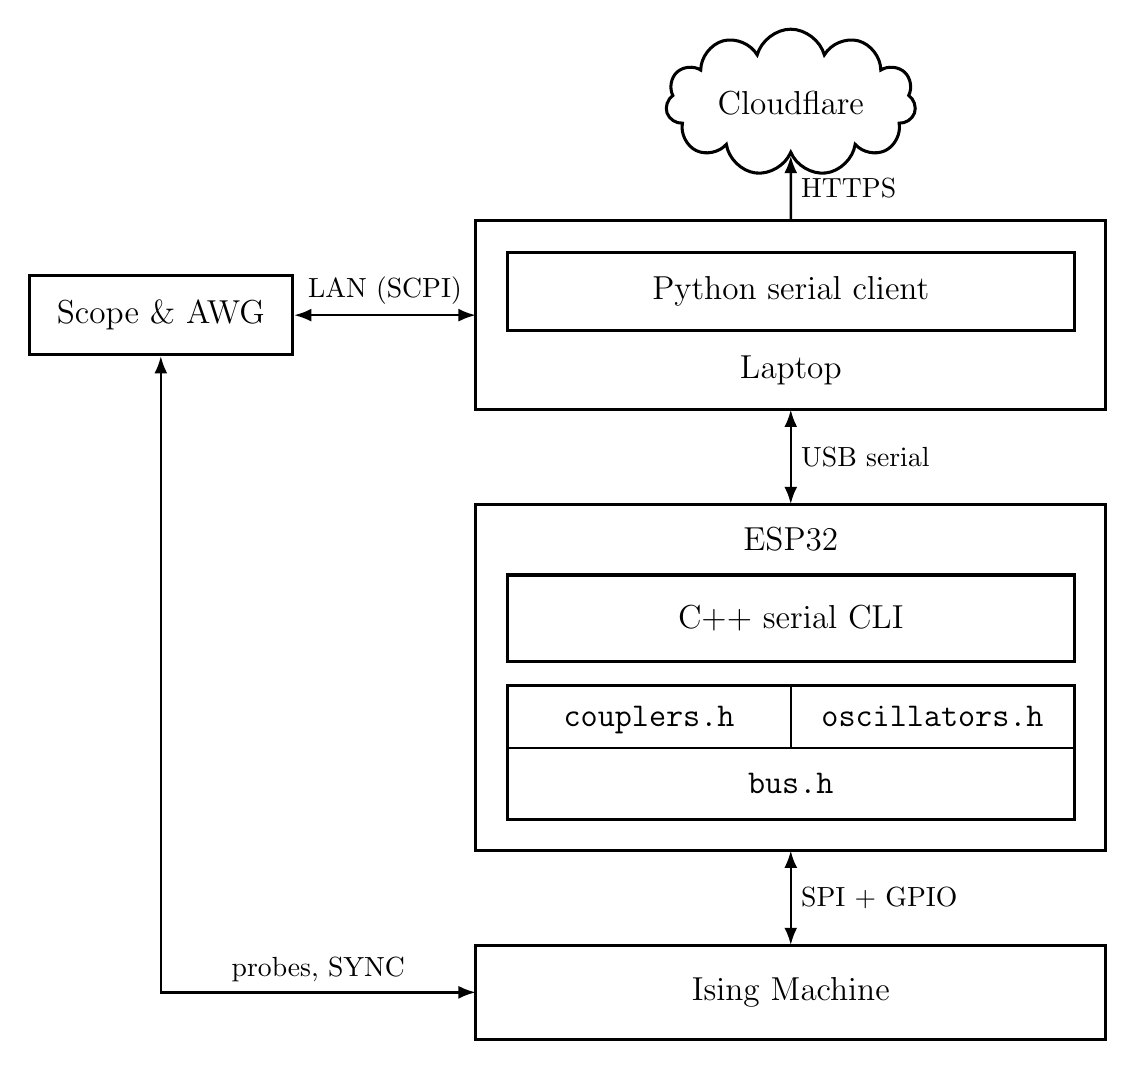
\begin{tikzpicture}[
    font=\large, line width=0.9pt, >={Latex[length=2.2mm]},
    box/.style={draw, line width=1.1pt, align=center},
    lbl/.style={font=\normalsize},
  ]
  % Cloudflare
  \node[draw, line width=1.1pt, cloud, cloud puffs=11, aspect=2.4, inner sep=4pt] (cf) at (5.0,2.9) {Cloudflare};

  % Laptop
  \draw[box] (1.0,1.4) rectangle (9.0,-1.0);
  \draw[box] (1.4,1.0) rectangle (8.6,0.0);
  \node at (5.0,0.5) {Python serial client};
  \node at (5.0,-0.5) {Laptop};
  \draw[->] (5.0,1.4) -- node[lbl, right] {HTTPS} (cf.south);

  % Scope & AWG
  \node[box, minimum height=1.0cm, inner xsep=10pt] (scope) at (-3.0,0.2) {Scope \& AWG};
  \draw[<->] (scope.east) -- node[lbl, above] {LAN (SCPI)} (1.0,0.2);
  \draw[<->] (scope.south) |- node[lbl, pos=0.75, above] {probes, SYNC} (1.0,-8.4);

  % ESP32
  \draw[box] (1.0,-2.2) rectangle (9.0,-6.6);
  \node at (5.0,-2.65) {ESP32};
  \draw[box] (1.4,-3.1) rectangle (8.6,-4.2);
  \node at (5.0,-3.65) {C++ serial CLI};
  \draw[box] (1.4,-4.5) rectangle (8.6,-6.2);
  \draw (1.4,-5.3) -- (8.6,-5.3) (5.0,-4.5) -- (5.0,-5.3);
  \node[font=\large\ttfamily, anchor=base] at (3.2,-5.02) {couplers.h};
  \node[font=\large\ttfamily, anchor=base] at (6.8,-5.02) {oscillators.h};
  \node[font=\large\ttfamily] at (5.0,-5.75) {bus.h};
  \draw[<->] (5.0,-1.0) -- node[lbl, right] {USB serial} (5.0,-2.2);

  % Ising machine
  \draw[box] (1.0,-7.8) rectangle (9.0,-9.0);
  \node at (5.0,-8.4) {Ising Machine};
  \draw[<->] (5.0,-6.6) -- node[lbl, right] {SPI + GPIO} (5.0,-7.8);
\end{tikzpicture}
\end{document}
